\documentclass[12pt]{article}
\usepackage[russian]{babel}
\usepackage[utf8x]{inputenc}
\usepackage{amssymb}
\usepackage{amsmath}
\usepackage{graphicx}
\usepackage{geometry}
\usepackage[colorinlistoftodos]{todonotes}
\usepackage{listings}
\usepackage[section]{placeins}
\begin{document}

\title{7. Спектральное оценивание при помощи периодограммного метода}
\author{Андрей Валиков}
\date{}
\maketitle
																																																							


\section{Формирование последовательности}


\[f = \sin(\omega_1 Tt) + \cos(\omega_2 Tt)\]


\begin{lstlisting}
N = 2 ** 11

teta = np.arange(0, N, 1)
T = .02
w1 = 81
w2 = 14
b = 5

f = np.sin(w1 * T * teta) + np.cos(w2 * T * teta)

r1 = b * np.random.rand(N)
r = r1 - np.mean(r1)

x = f + r;

plt.plot(teta, f)
plt.show()

plt.plot(teta, r)
plt.show()

plt.plot(teta, x)
plt.show()
\end{lstlisting}


\begin{figure}[!htb]
\centering
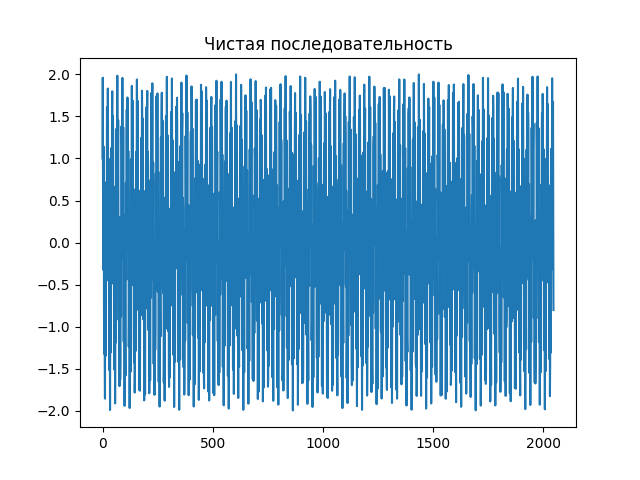
\includegraphics[scale=1.00]{good.png}
\caption{}
\label{}
\end{figure}

\begin{figure}[!htb]
\centering
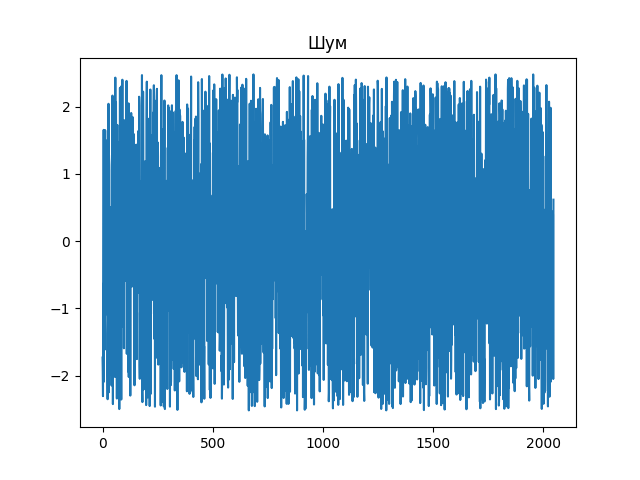
\includegraphics[scale=1.00]{bad.png}
\caption{}
\label{}
\end{figure}

\begin{figure}[!htb]
\centering
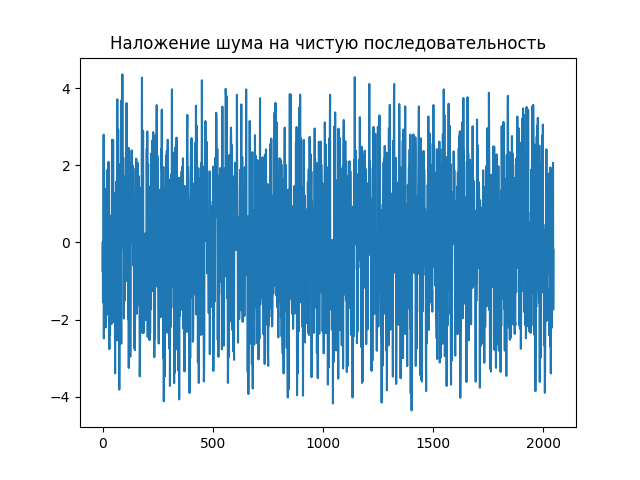
\includegraphics[scale=1.00]{ugly.png}
\caption{}
\label{}
\end{figure}


\section{Разбиение последовательности на сегменты}




\begin{lstlisting}
D = .5
L = int(N / 2)
V = int((N - D * L) / (L - D * L))
print(V)

teta1 = np.arange(0, L, 1)
x1 = np.zeros((V, L))

for i in range(L):
  x1[0, i] = x[i]
  x1[1, i] = x[i + 64]
  x1[2, i] = x[i + 128]

plt.plot(teta, x)
plt.show()

plt.plot(teta1, x1[0, :])
plt.show()

plt.plot(teta1, x1[1, :])
plt.show()

plt.plot(teta1, x1[2, :])
plt.show()
\end{lstlisting}



\begin{figure}[!htb]
\centering
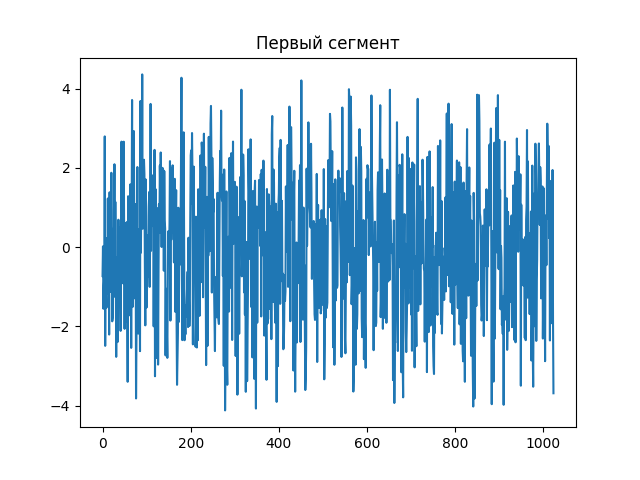
\includegraphics[scale=1.00]{first_seg.png}
\caption{}
\label{}
\end{figure}

\begin{figure}[!htb]
\centering
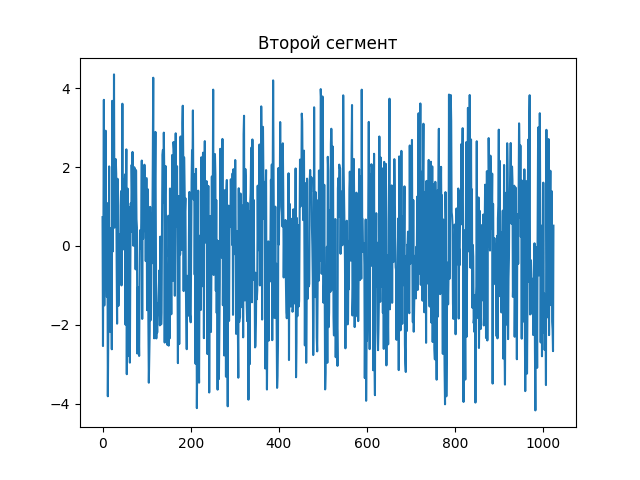
\includegraphics[scale=1.00]{second_seg.png}
\caption{}
\label{}
\end{figure}

\begin{figure}[!htb]
\centering
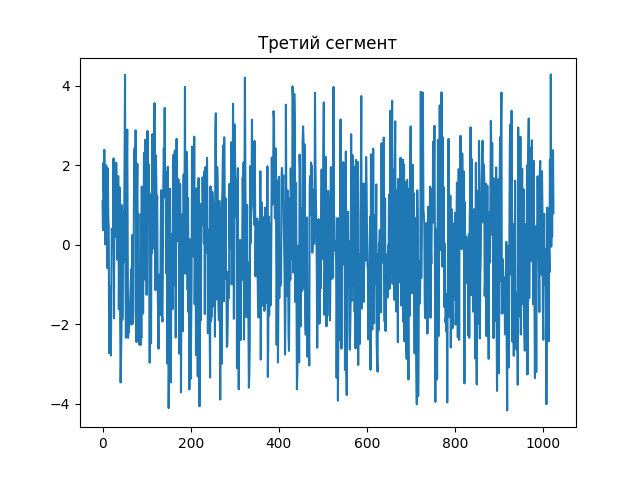
\includegraphics[scale=1.00]{third_seg.png}
\caption{}
\label{}
\end{figure}

\section{ Нахождение спектральных характеристик и периодограмм}

\begin{lstlisting}
w = np.zeros(L)
for i in range(L):
    if 0 <= teta[i] <= (L - 1) / 2:
        w[i] = 2 * teta[i] / (L - 1)

    else:
        w[i] = 2 - (2 * teta[i]) / (L - 1)

plt.plot(teta1, w);
plt.show()


y = np.zeros((V, L))
for i in range(V):
  for j in range(L):
    y[i, j] = x1[i, j] * w[j]

S = np.zeros((V, L))

for i in range(V):
  S[i, :] = np.fft.fft(y[i, :])

plt.plot(teta1, S[0,:])
plt.show()

plt.plot(teta1, S[1,:])
plt.show()

plt.plot(teta1, S[2,:])
plt.show()

P = np.zeros((V, L))
for i in range(V):
  for j in range(L):
    P[i, j] = (1 / N) * S[i, j] ** 2;

plt.plot(teta1, P[0,:])
plt.show()

plt.plot(teta1, P[1,:])
plt.show()

plt.plot(teta1, P[2,:])
plt.show()
\end{lstlisting}

\begin{figure}[!htb]
\centering
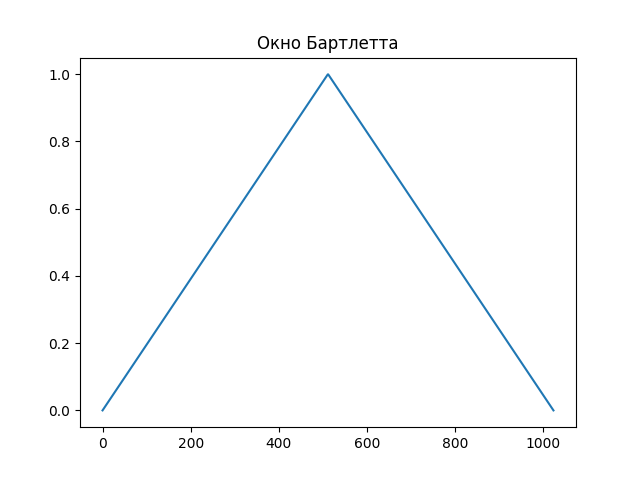
\includegraphics[scale=1.00]{bart_window.png}
\caption{}
\label{}
\end{figure}

\begin{figure}[!htb]
\centering
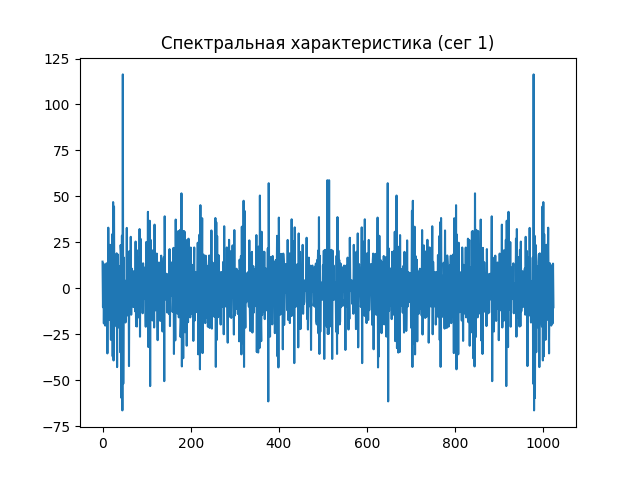
\includegraphics[scale=1.00]{spec_1.png}
\caption{}
\label{}
\end{figure}

\begin{figure}[!htb]
\centering
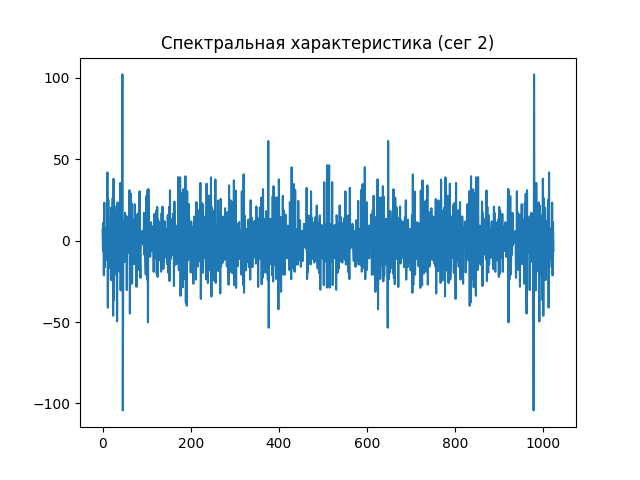
\includegraphics[scale=1.00]{spec_2.png}
\caption{}
\label{}
\end{figure}

\begin{figure}[!htb]
\centering
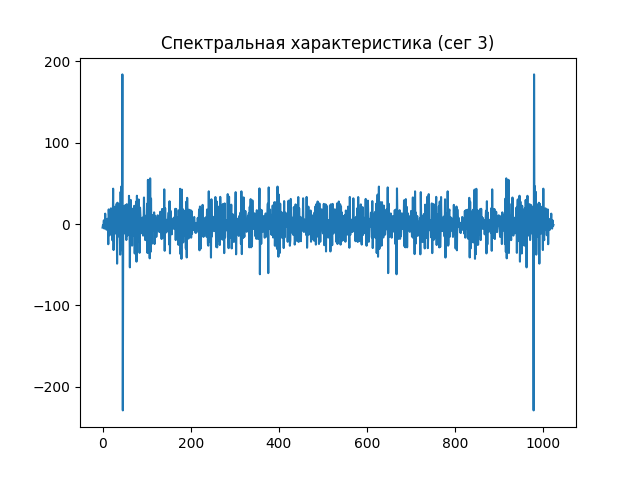
\includegraphics[scale=1.00]{spec_3.png}
\caption{}
\label{}
\end{figure}



\begin{figure}[!htb]
\centering
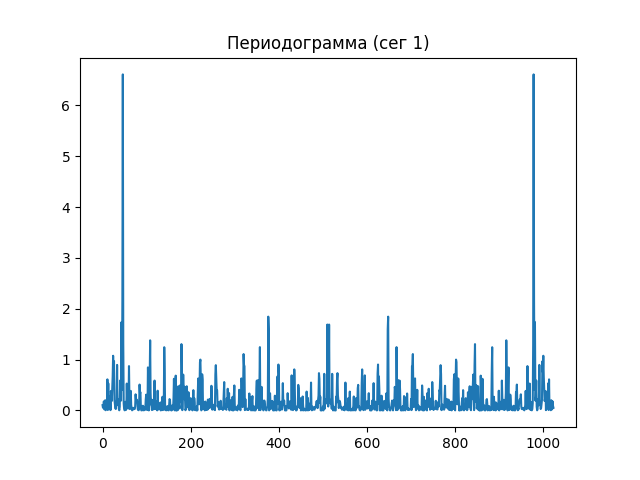
\includegraphics[scale=1.00]{period_1.png}
\caption{}
\label{}
\end{figure}

\begin{figure}[!htb]
\centering
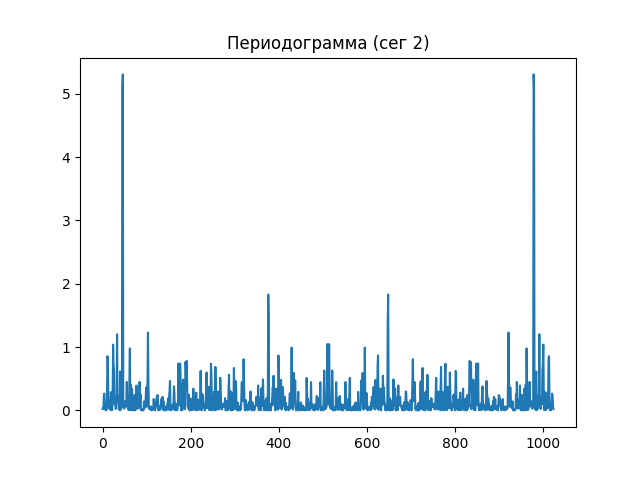
\includegraphics[scale=1.00]{period_2.png}
\caption{}
\label{}
\end{figure}


\begin{figure}[!htb]
\centering
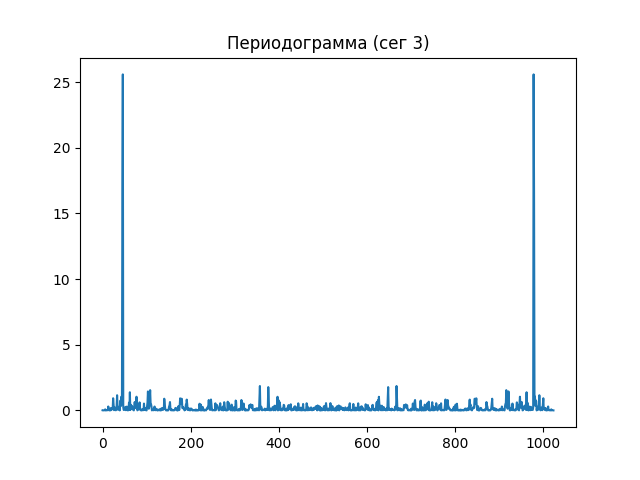
\includegraphics[scale=1.00]{period_3.png}
\caption{}
\label{}
\end{figure}



\section{Получение оценки спектральной мощности для каждого сегмента}

\begin{lstlisting}
def Search(S, T, number):
  ix = S > number
  mask(2:length(ix) + 1) = ix
  nd = find(mask)

  k1 = np.ceil(abs(S(nd[0])))
  k2 = np.ceil(abs(S(nd[1])))

  w1 = np.pi * k1/(512 * T)
  w2 = np.pi * k2/(512 * T)
  ww = [w1 w2]
  return ww

ww1 = Search(S[0, :], T, 200)
ww2 = Search(S[1, :], T, 95)
ww3 = Search(S[2, :], T, 200)

print(ww1)
print(ww2)
print(ww3)
\end{lstlisting}


$\omega_1$ = 38.96  
$\omega_2$ = 29.14

$\omega_1$ = 81.6
$\omega_2$ = 6.13

$\omega_1$ = 40.8   
$\omega_2$ = 33.75

\section{Вывод}
Изучен периодограммный метод оценивания спектральной плотности. Получена тестовая последовательность дискретных значений с наложенным на неё случайным процессом. Последовательность была разбита на 3 сегмента. Количество сегментов было получено по заданной формуле. Далее была выбрана оконная функция Барлетта и найдена спектральная характеристика и периодограммы для каждого сегмента.
В результате работы программы были получены следующие угловые частоты:\\

Для первого сегмента:\\
$\omega_1$ = 38.96  
$\omega_2$ = 29.14\\

Для второго сегмента:\\
$\omega_1$ = 81.6
$\omega_2$ = 6.13\\

Для третьего сегмента:\\
$\omega_1$ = 40.8   
$\omega_2$ = 33.75

\end{document}